\documentclass{article}
\usepackage{graphicx}
\usepackage{multicol}
\usepackage[margin=0.5in]{geometry}
\begin{document}
\title{Matching Trig Graphs A}
\maketitle
\noindent
Write the name of the graph that matches the given equation. Use only
your unit circle (or knowledge thereof) to complete this activity.
\begin{multicols}{2}
\begin{enumerate}
	\item $y=\sin x$ \hspace{1cm} \rule{5cm}{0.5pt}
	\item $y=\cos x$ \hspace{1cm} \rule{5cm}{0.5pt}
	\item $y=\tan x$ \hspace{1cm} \rule{5cm}{0.5pt}
	\item $y=\csc x$ \hspace{1cm} \rule{5cm}{0.5pt}
	\item $y=\sec x$ \hspace{1cm} \rule{5cm}{0.5pt}
	\item $y=\cot x$ \hspace{1cm} \rule{5cm}{0.5pt}
\end{enumerate}

\noindent
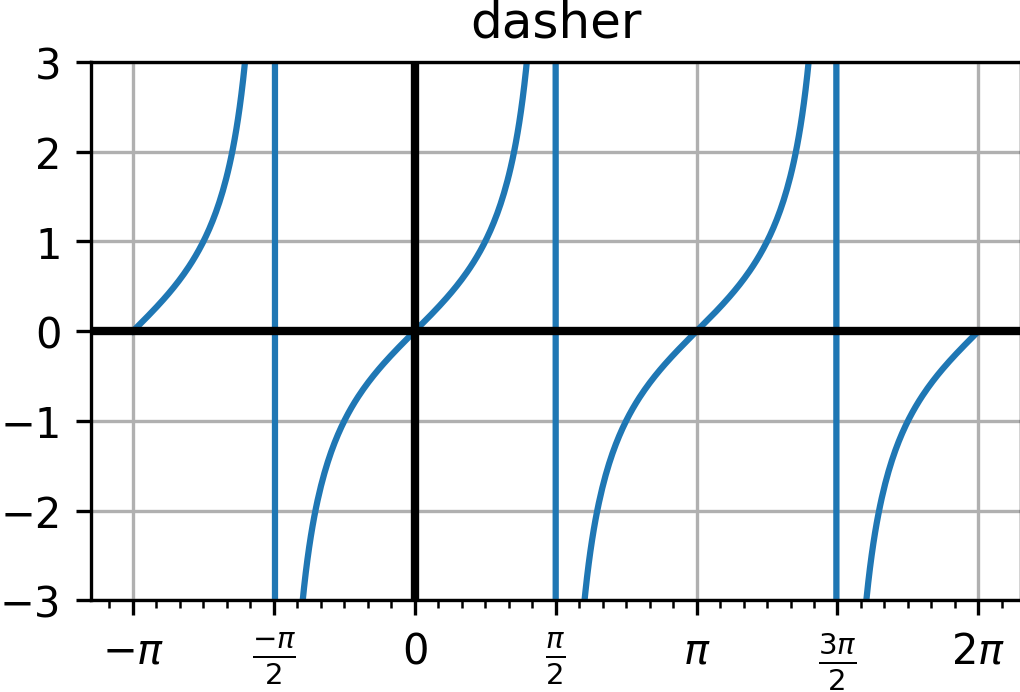
\includegraphics[width=3in]{dasher.png} \\
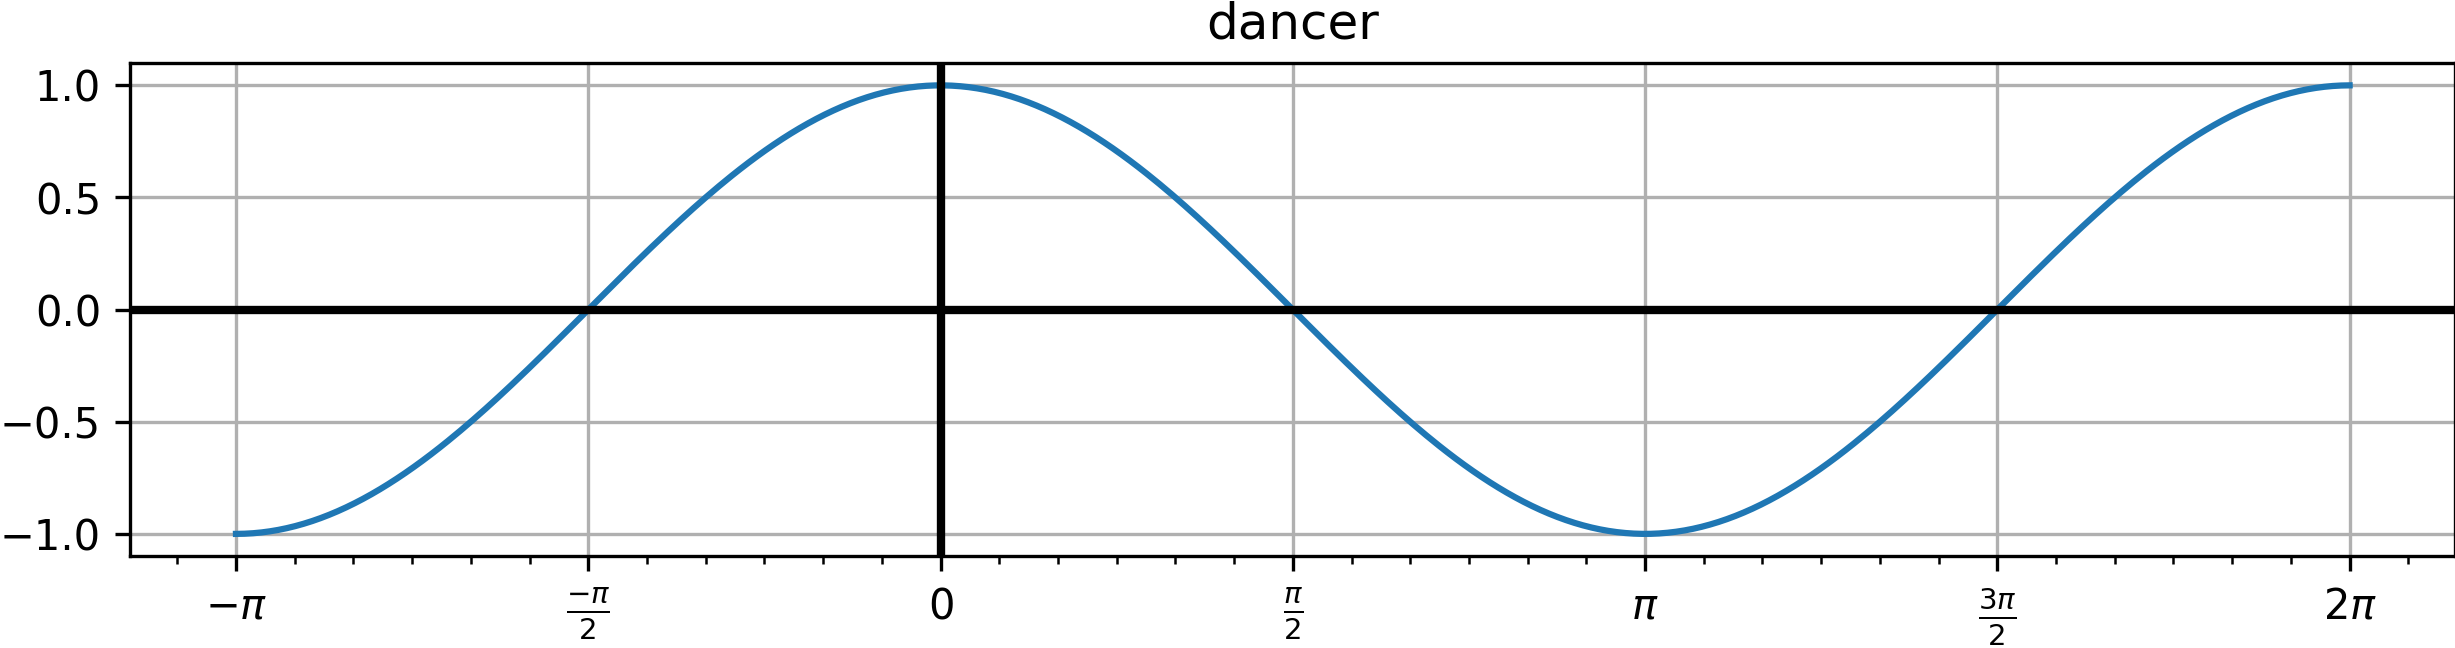
\includegraphics[width=3in]{dancer.png} \\
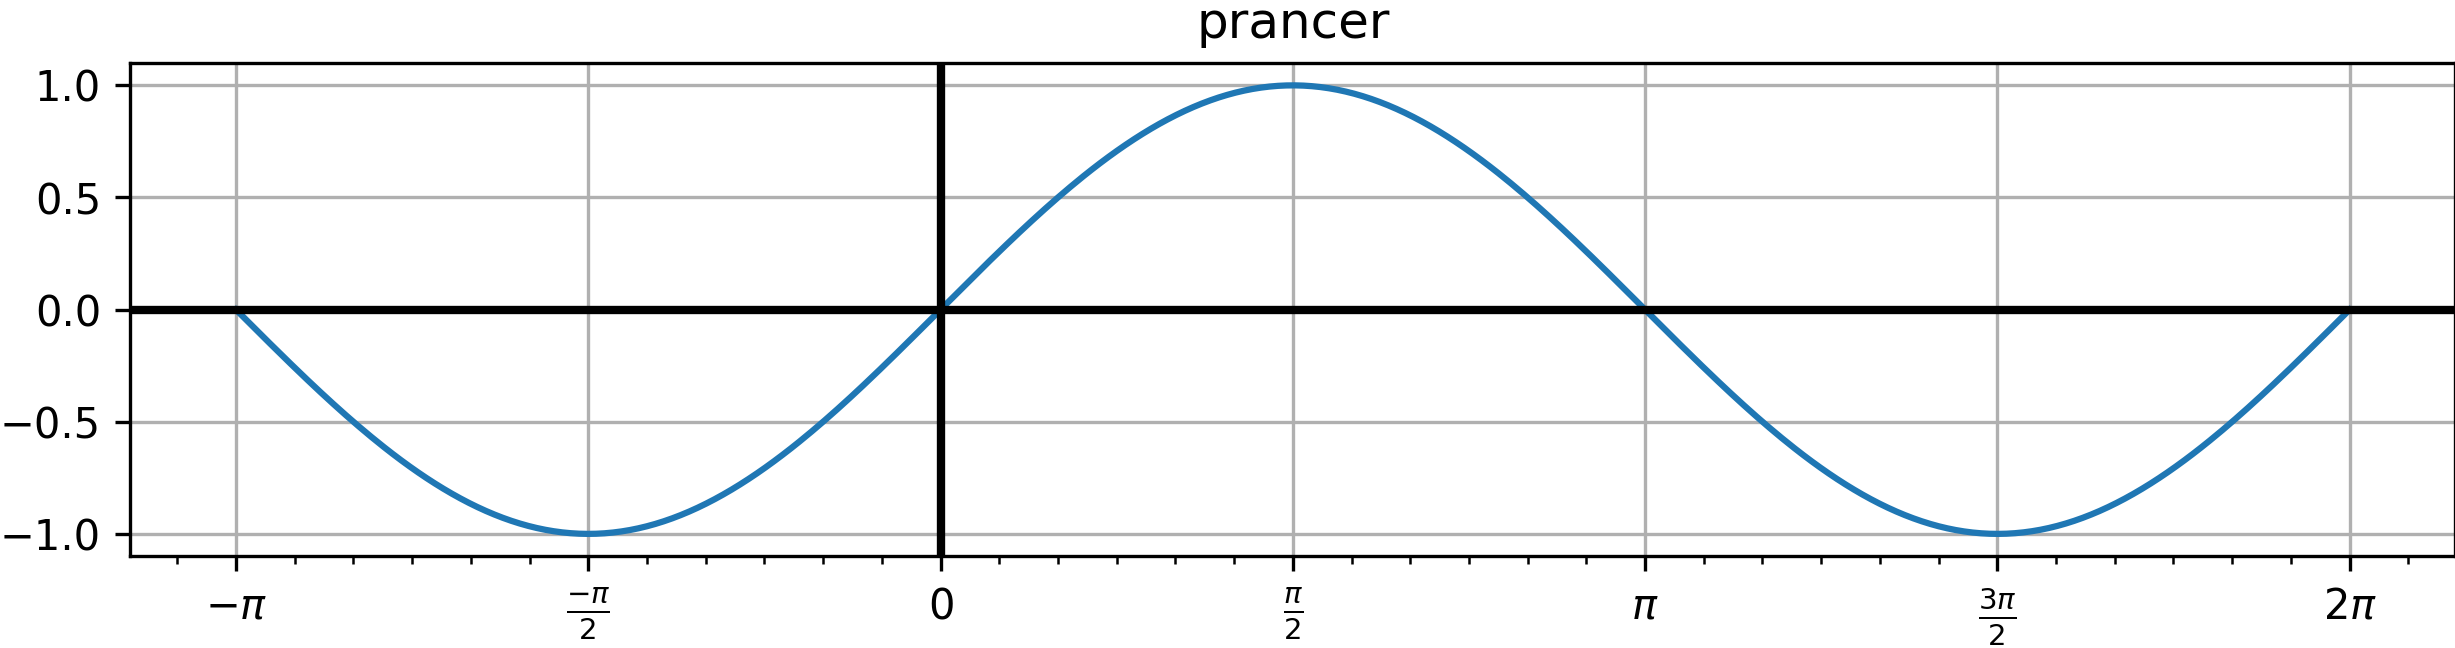
\includegraphics[width=3in]{prancer.png} \\
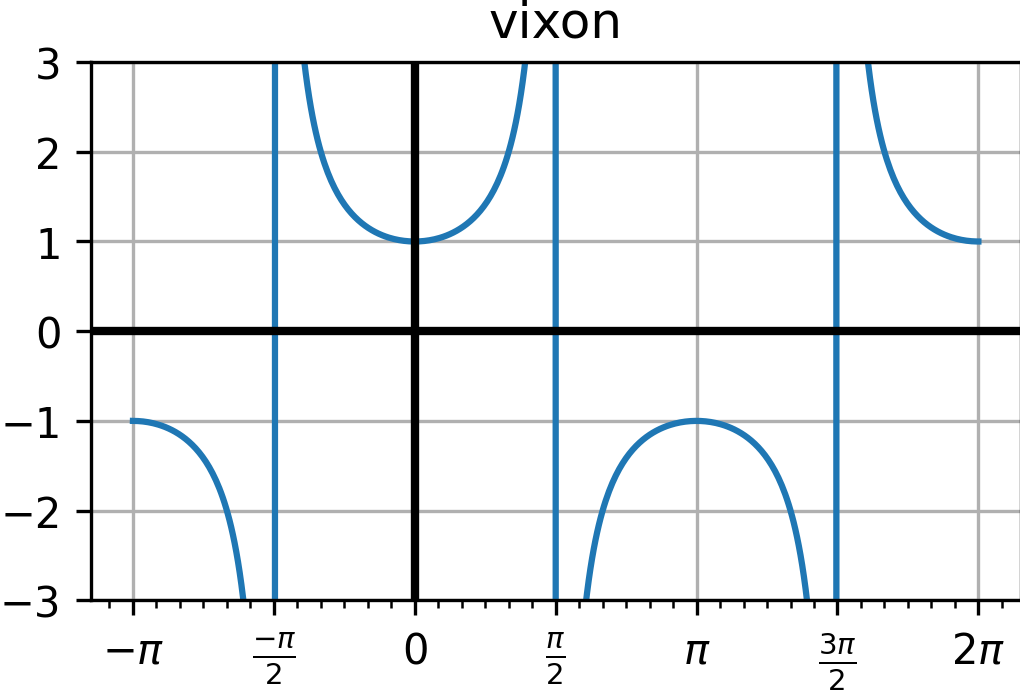
\includegraphics[width=3in]{vixon.png} \\
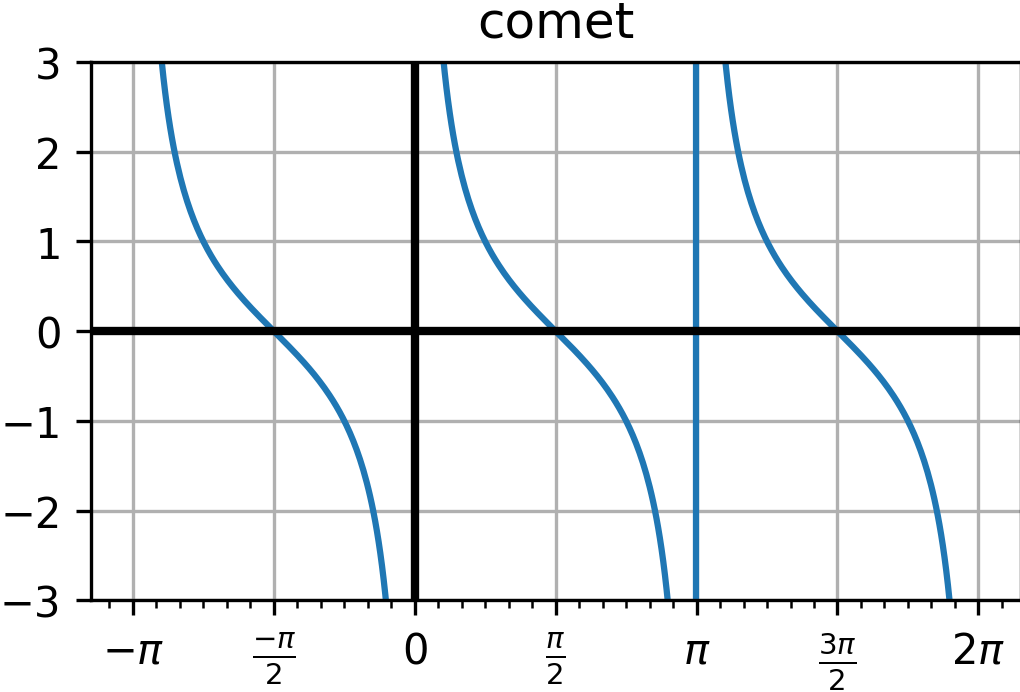
\includegraphics[width=3in]{comet.png} \\
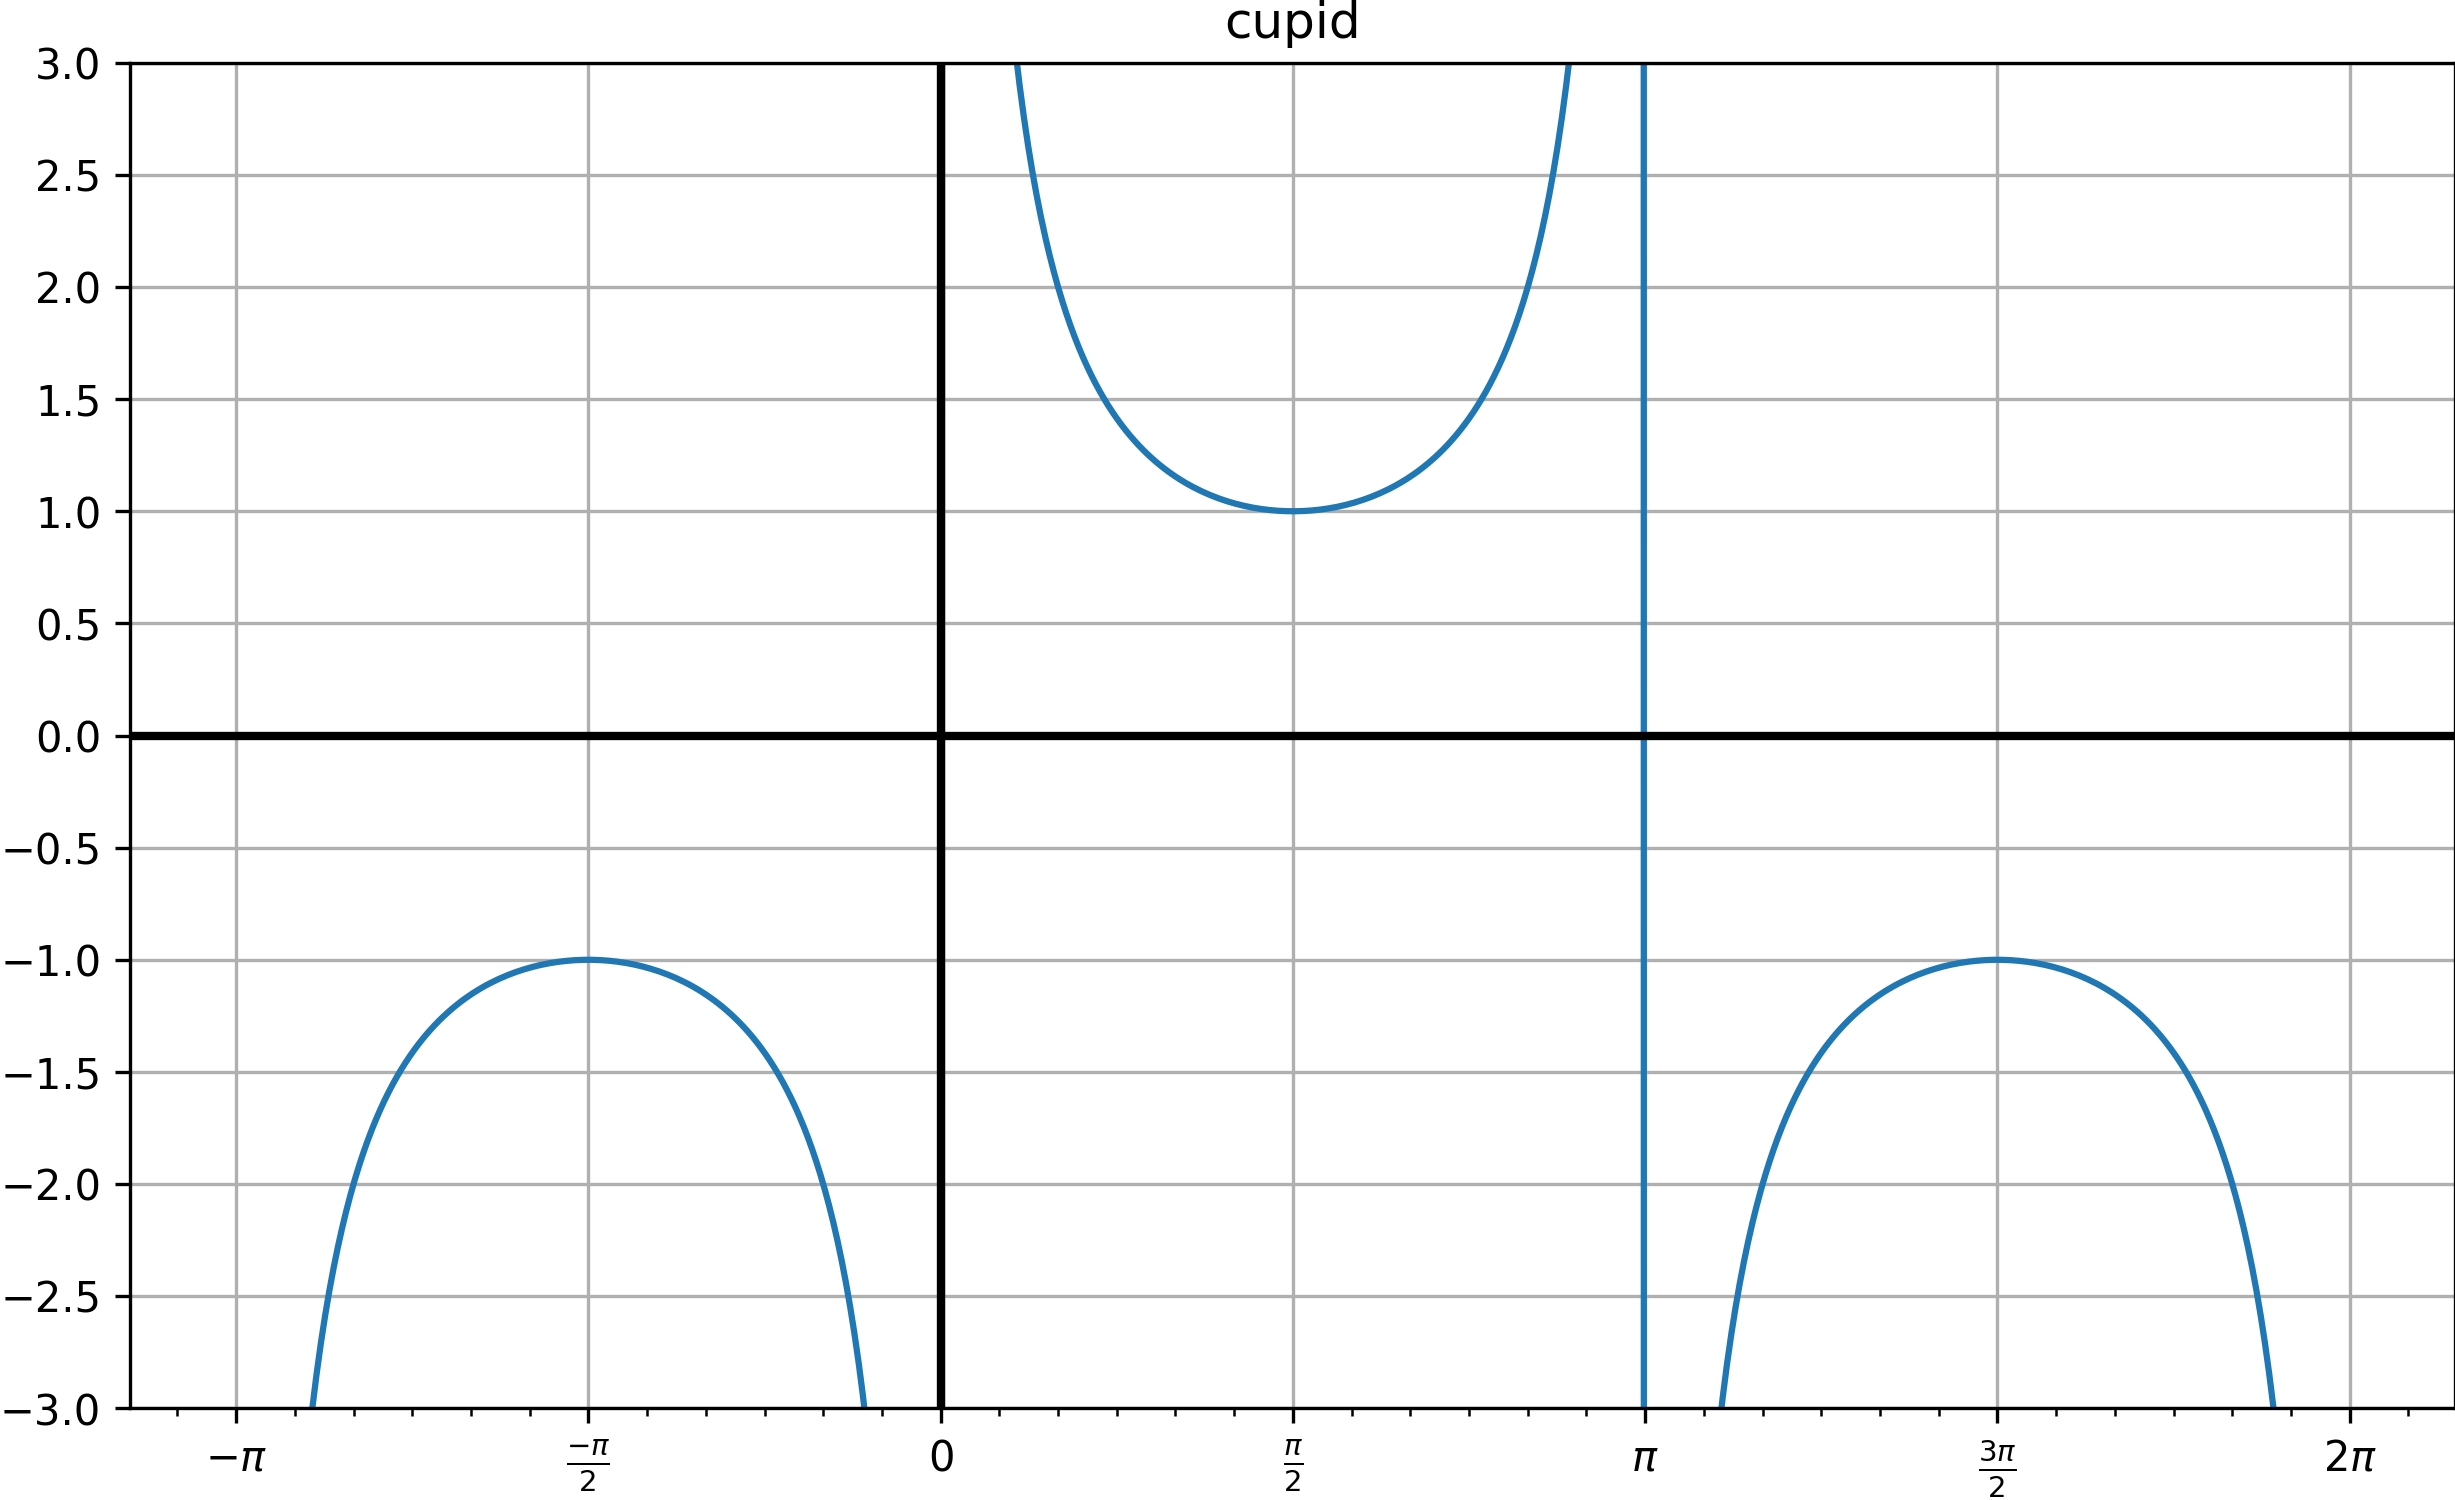
\includegraphics[width=3in]{cupid.png}
\end{multicols}
\end{document}
